% A LaTeX template for EXECUTIVE SUMMARY of the MSc Thesis submissions to
% Politecnico di Milano (PoliMi) - School of Industrial and Information Engineering
%
% P. F. Antonietti, S. Bonetti, A. Gruttadauria, G. Mescolini, A. Zingaro
% e-mail: template-tesi-ingind@polimi.it
%
% Last Revision: October 2021
%
% Copyright 2021 Politecnico di Milano, Italy. Inc. All rights reserved.

\documentclass[11pt,a4paper]{article}

%------------------------------------------------------------------------------
%	REQUIRED PACKAGES AND  CONFIGURATIONS
%------------------------------------------------------------------------------
% PACKAGES FOR TITLES
\usepackage{titlesec}
\usepackage{color}
% PACKAGES FOR LANGUAGE AND FONT
\usepackage[utf8]{inputenc}
\usepackage[english]{babel}
\usepackage[T1]{fontenc} % Font encoding
\usepackage{lmodern} % Latin Modern font
% PACKAGES FOR IMAGES
\usepackage{graphicx}
\graphicspath{{Images/}} % Path for images' folder
\usepackage{eso-pic} % For the background picture on the title page
\usepackage{subfig} % Numbered and caption subfigures using \subfloat
\usepackage{caption} % Coloured captions
%\usepackage{subcaption}
\usepackage{transparent}

% STANDARD MATH PACKAGES
\usepackage{amsmath}
\usepackage{amsthm}
\usepackage{bm}
\usepackage[overload]{empheq}  % For braced-style systems of equations

% PACKAGES FOR TABLES
\usepackage{tabularx}
\usepackage{longtable} % tables that can span several pages
\usepackage{colortbl}

% PACKAGES FOR ALGORITHMS (PSEUDO-CODE)
\usepackage{algorithm}
\usepackage{algorithmic}
% PACKAGES FOR REFERENCES & BIBLIOGRAPHY
\usepackage{biblatex} %Imports biblatex package
\addbibresource{mimesis.bib}
\usepackage[colorlinks=true,linkcolor=black,anchorcolor=black,citecolor=black,filecolor=black,menucolor=black,runcolor=black,urlcolor=black]{hyperref} % Adds clickable links at references
\usepackage{cleveref}
%\usepackage[square, numbers, sort&compress]{natbib} % Square brackets, citing references with numbers, citations sorted by appearance in the text and compressed
\usepackage{bookmark} % Add this package to fix the reported errors
% \bibliographystyle{plain} % You may use a different style adapted to your field
% \bibliographystyle{plain} % You may use a different style adapted to your field

% PACKAGES FOR THE APPENDIX
\usepackage{appendix}

% PACKAGES FOR ITEMIZE & ENUMERATES
\usepackage{enumitem}

% OTHER PACKAGES
\usepackage{amsthm,thmtools,xcolor} % Coloured "Theorem"
\usepackage{comment} % Comment part of code
\usepackage{fancyhdr} % Fancy headers and footers
\usepackage{lipsum} % Insert dummy text
\usepackage{tcolorbox} % Create coloured boxes (e.g. the one for the key-words)
\usepackage{stfloats} % Correct position of the tables
\usepackage{multirow}
\usepackage{multicol}





%-------------------------------------------------------------------------
%	NEW COMMANDS DEFINED
%-------------------------------------------------------------------------
% EXAMPLES OF NEW COMMANDS -> here you see how to define new commands
\newcommand{\bea}{\begin{eqnarray}} % Shortcut for equation arrays
\newcommand{\eea}{\end{eqnarray}}
\newcommand{\e}[1]{\times 10^{#1}}  % Powers of 10 notation
\newcommand{\mathbbm}[1]{\text{\usefont{U}{bbm}{m}{n}#1}} % From mathbbm.sty
\newcommand{\pdev}[2]{\frac{\partial#1}{\partial#2}}
% NB: you can also override some existing commands with the keyword \renewcommand

%----------------------------------------------------------------------------
%	ADD YOUR PACKAGES (be careful of package interaction)
%----------------------------------------------------------------------------
\usepackage{amsfonts} 
\usepackage[font=footnotesize,labelfont=bf]{caption}

%----------------------------------------------------------------------------
%	ADD YOUR DEFINITIONS AND COMMANDS (be careful of existing commands)
%----------------------------------------------------------------------------
\usepackage{import}
\usepackage{xifthen}
\usepackage{pdfpages}
\usepackage{transparent}
\usepackage{wrapfig}
\usepackage{dsfont}
\usepackage{shadethm}

\parindent=0pt

\newcommand{\incfig}[1]{%
    \def\svgwidth{\columnwidth}
    \import{./Images/}{#1.pdf_tex}
}
\newcommand*{\oldepsilon}{\epsilon}
\renewcommand*{\epsilon}{\varepsilon}
\DeclareMathOperator*{\esssup}{ess\,sup}

\numberwithin{equation}{section}
%----------------------------------------------------------------------------
%	CONFIGURATION OF THEOREM ENVIRONMENTS


% \newtheoremstyle{break}
%     {\partopsep}{\topsep}%  
%     {\normalfont}{}
%     {\bfseries}{}%
%     {\newline}{}%
% \theoremstyle{break}
% \newtheorem{theorem}{Theorem}[section]
% \newtheorem{corollary}{Corollary}[section]
% \newtheorem{proposition}{Proposition}[section]
% \newtheorem{remark}{Remark}[section]
% \newtheorem{lemma}{Lemma}[section]
% \newtheorem{notation}{Notation}[section]
% \newtheorem{definition}{Definition}[section]

% \newtheorem{definition}{Definition}[section]

% \newtheorem*{remark}{Remark}

% \newtheorem{lemma}{Lemma}[section]
% %----------------------------------------------------------------------------

% Do not change Configuration_files/config.tex file unless you really know what you are doing.
% This file ends the configuration procedures (e.g. customizing commands, definition of new commands)
% Set the geometric layout of the document
\usepackage{geometry}
\geometry{
  top=3cm,
  left = 2.0cm,
  right = 2.0cm,
  bottom=2cm,
  headheight= 2cm,
  headsep= 0cm,
}
\raggedbottom

% Create color bluePoli (-> manuale grafica coordinata:  https://www.polimi.it/fileadmin/user_upload/il_Politecnico/grafica-coordinata/2015_05_11_46xy_manuale_grafica_coordinata.pdf)
\definecolor{bluePoli}{cmyk}{0.4,0.1,0,0.4}

% Custom theorem environments
\declaretheoremstyle[
  shaded={rulecolor=bluePoli!20, rulewidth=1pt, bgcolor=bluePoli!5},
  headfont=\color{bluePoli}\normalfont\bfseries,
  bodyfont=\color{black}\normalfont,
]{colored}

\captionsetup[figure]{labelfont={color=bluePoli}} % Set colour of the captions
\captionsetup[table]{labelfont={color=bluePoli}} % Set colour of the captions
\captionsetup[algorithm]{labelfont={color=bluePoli}} % Set colour of the captions

\theoremstyle{colored}
\newtheorem{theorem}{Theorem}[section]
\newtheorem{proposition}{Proposition}[section]
\newtheorem{definition}{Definition}[section]
\newtheorem*{remark}{Remark}
\newtheorem{lemma}{Lemma}[section]

% Enhances the features of the standard "table" and "tabular" environments.
\newcommand\T{\rule{0pt}{2.6ex}}
\newcommand\B{\rule[-1.2ex]{0pt}{0pt}}

% Algorithm description
\newcounter{algsubstate}
\renewcommand{\thealgsubstate}{\alph{algsubstate}}
\newenvironment{algsubstates}{
    \setcounter{algsubstate}{0}%
    \renewcommand{\STATE}{%
    \stepcounter{algsubstate}%
    \Statex {\small\thealgsubstate:}\space}
    }{}

% Custom theorem environment
\newcolumntype{L}[1]{>{\raggedright\let\newline\\\arraybackslash\hspace{0pt}}m{#1}}
\newcolumntype{C}[1]{>{\centering\let\newline\\\arraybackslash\hspace{0pt}}m{#1}}
\newcolumntype{R}[1]{>{\raggedleft\let\newline\\\arraybackslash\hspace{0pt}}m{#1}}

% Custom itemize environment
\setlist[itemize,1]{label=$\bullet$}
\setlist[itemize,2]{label=$\circ$}
\setlist[itemize,3]{label=$-$}
\setlist{nosep}

% Set separation of columns
\setlength{\columnsep}{30pt}

% Create command for background pic
\newcommand\BackgroundPic{% Adding background picture
	\put(230,358){
		\parbox[b][\paperheight]{\paperwidth}{%
			\vfill
			\centering
			\transparent{0.2}
			
\includegraphics[width=0.8\paperwidth]{raggiera_polimi.eps}%
			\vfill
}}}

% Set indentation
%\setlength\parindent{0pt}

% Custom title commands
\titleformat{\section}
{\color{bluePoli}\normalfont\Large\bfseries}
{\color{bluePoli}\thesection.}{1em}{}
\titlespacing*{\section}
{0pt}{2ex}{1ex}

\titleformat{\subsection}
{\color{bluePoli}\normalfont\large\bfseries}
{\color{bluePoli}\thesubsection.}{1em}{}
\titlespacing*{\subsection}
{0pt}{2ex}{1ex}

\titleformat{\subsubsection}
{\color{bluePoli}\normalfont\normalsize\bfseries}
{\color{bluePoli}\thesubsubsection.}{1em}{}
\titlespacing*{\subsubsection}
{0pt}{2ex}{1ex}

% Custom headers and footers
\pagestyle{fancy}
\fancyhf{}

\fancyfoot{}
\fancyfoot[C]{\thepage} % page
\renewcommand{\headrulewidth}{0mm} % headrule width
\renewcommand{\footrulewidth}{0mm} % footrule width

\makeatletter
\patchcmd{\headrule}{\hrule}{\color{black}\hrule}{}{} % headrule
\patchcmd{\footrule}{\hrule}{\color{black}\hrule}{}{} % footrule
\makeatother

% -> Create the header
\chead[C]{
\centering
\begin{tcolorbox}[arc=0pt, boxrule=0pt, colback=bluePoli!60, width=\textwidth, colupper=white]
    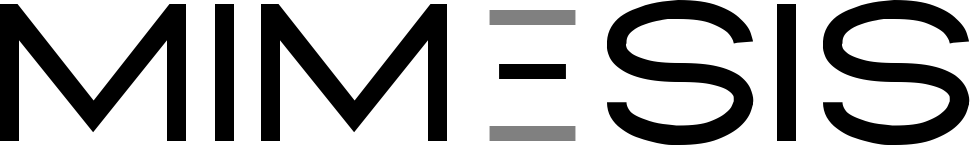
\includegraphics[width=0.2\textwidth]{mimesis.png}
\end{tcolorbox}
}


% Insert here the info that will be displayed into your Title page
% -> title of your work
\renewcommand{\title}{\noindent Accelerating Numerical Simulation:

a Data-Driven correction of Finite Element Methods}

% -> author name and surname
\renewcommand{\author}{Andrea Bonifacio}
% -> MSc course
\newcommand\norm[1]{\lVert#1\rVert}
\newcommand{\course}{Mimesis Team}
% -> advisor name and surname
\newcommand{\advisor}{Stéphane Cotin}
% IF AND ONLY IF you need to modify the co-supervisors you also have to modify the file Configuration_files/title_page.tex (ONLY where it is marked)
%\newcommand{\firstcoadvisor}{Name Surname} % insert if any otherwise comment
%\newcommand{\secondcoadvisor}{Name Surname} % insert if any otherwise comment
% -> academic year
\newcommand{\YEAR}{2023-2024}


%-------------------------------------------------------------------------
%	BEGIN OF YOUR DOCUMENT
\usepackage{bookmark} % Add this package to fix the reported errors

\begin{document}
%-----------------------------------------------------------------------------
% TITLE PAGE
%-----------------------------------------------------------------------------
% Do not change Configuration_files/TitlePage.tex (Modify it IF AND ONLY IF you need to add or delete the Co-advisors)
% This file creates the Title Page of the document
% DO NOT REMOVE SPACES BETWEEN LINES!

%\twocolumn[{\begin{@twocolumnfalse}

\AddToShipoutPicture*{\BackgroundPic}

\hspace{-0.6cm}
\includegraphics[width=0.6\textwidth]{logo_polimi_ing_indinf.eps}

\vspace{-1mm}
\fontsize{0.3cm}{0.5cm}\selectfont \bfseries \textsc{\color{bluePoli} Report}\\

\vspace{-0.2cm}
\Large{\textbf{\color{bluePoli}{\title}}}\\

\vspace{-0.2cm}
\fontsize{0.3cm}{0.5cm}\selectfont \bfseries \textsc{\color{bluePoli} \course}\\

\vspace{-0.2cm}
\fontsize{0.3cm}{0.5cm} \selectfont \bfseries Authors: \textsc{\textbf{\author}}\\

%\vspace{-0.4cm}
%\fontsize{0.3cm}{0.5cm}\selectfont \bfseries Advisor: \textsc{\textbf{\advisor}}\\

% if only ONE co-advisor is present:
%\vspace{-0.4cm}
%\fontsize{0.3cm}{0.5cm}\selectfont \bfseries Co-advisor: \textsc{\textbf{\firstcoadvisor}}\\
% if more than one co-advisors are present:
%\vspace{-0.4cm}
%\fontsize{0.3cm}{0.5cm}\selectfont \bfseries Co-advisors: \textsc{\textbf{\firstcoadvisor}}\textsc{\textbf{\secondcoadvisor}}\\

\vspace{-0.4cm}
\fontsize{0.3cm}{0.5cm}\selectfont \bfseries Academic year: \textsc{\textbf{\YEAR}}

\small \normalfont

\vspace{11pt}

\centerline{\rule{1.0\textwidth}{0.4pt}}

%\vspace{15pt}
%\end{@twocolumnfalse}}]

\thispagestyle{plain} % In order to not show the header in the first page


%%%%%%%%%%%%%%%%%%%%%%%%%%%%%%
%%     THESIS MAIN TEXT     %%
%%%%%%%%%%%%%%%%%%%%%%%%%%%%%%


%-----------------------------------------------------------------------------
% INTRODUCTION
%-----------------------------------------------------------------------------

\section{Introduction}

Numerical simulations play a critical role in a wide array of scientific and engineering applications, providing insights into the behavior of physical systems under various conditions. Among the most prominent techniques for performing such simulations is Finite Element Modeling (FEM). FEM discretizes a continuous domain into a mesh of finite elements, allowing for the approximation of solutions to complex partial differential equations (PDEs). However, one significant drawback of FEM is its computational intensity, especially when high resolution is required for accurate results. This research aims to explore the potential of Deep Learning (DL) techniques to accelerate FEM simulations, focusing specifically on the deformation of objects subjected to external forces.

The deformation of an object under an applied force is directly tied to the object's discretization. In FEM, the object is represented by a mesh, where the resolution of the mesh—i.e., the size and number of elements—clearly impacts the accuracy and computational cost of the simulation. High-resolution meshes can capture fine details of deformation, leading to more accurate simulations, but they are computationally expensive and time-consuming. 

The main goal of this work is to study the efficacy of a method that combines both Finite Element Modeling (FEM) and DL to obtain a realistic simulation of an object in a fraction of the time that would be required by a traditional FEM simulation. The idea is to, somehow, train a DL model to have inside the information given by the refined discretization and pass them on a coarser discretization.

The idea of using DL techniques to solve scientific problem is not new. Thanks to the rise of new frameworks and libraries, such as TensorFlow and PyTorch, it is now possible to train very complex models on large datasets in a reasonable amount of time. For the problem at hand, a lot of different approaches can be found in the existing literature: a lot of them are based on the idea that the deep learning model should predict the whole dynamic of the system, for example MeshGraphNet \cite{pfaffLearningMeshBasedSimulation2021a} or its multiscale version \cite{fortunatoMultiScaleMeshGraphNets2022}, but these are just two examples of the many possible approaches \cite{jiangMeshfreeFlowNetPhysicsConstrainedDeep2020}, \cite{djeumouNeuralNetworksPhysicsInformed2022}, \cite{hanPredictingPhysicsMeshreduced2022a}. Other methods rely on solving a time independent problem, using various architectures, such as PINNs \cite{djeumouNeuralNetworksPhysicsInformed2022} or GNNs \cite{gaoPhysicsinformedGraphNeural2022}. The proposed method falls into the second category, as it will be explained in the following sections.

One interesting solution is given by \cite{Wang_Du_Coros_Thomaszewski_2024}, where the authors extend the concept of linear modes and modal dynamics \cite{Pentland_Williams_1989} to be able to handle larger deformations. The key idea is to obtain a linear approximation of the deformation, then train a network to minimize the energy of the system, so that for every modal coordinate, the network will learn a non-linear correction, effectively learning a series of non-linear modes. This allows for faster simulations by exploiting subspace dynamics, where the simulation is performed in a reduced space to ease computational costs. The authors show that 



\section{Problem setting}
In this section will be outlined a mathematical description of the problem. It will be divided in the two case under study: the static case and the dynamic case.

\subsection{Static case}
The static case is the simplest one. In this case we have a domain $\Omega \subset \mathbb{R}^d$ with $d=2,3$ and a force $f$ acting on it. A Lagrangian description of the problem is considered, where the material coordinates are given by the vector $\bm{X}$ and the deformed state of the solid is given by
\begin{equation}
    \bm{x} = \bm{X} + \bm{u}
\label{eq:deformation}
\end{equation}
where $\bm{u}$ is the displacement field. The model used to describe the linear relation between the stress tensor $\bm{\sigma} \in \mathbb{R}^{3\times 3}$ and the strain tensor $\bm{\varepsilon} \in \mathbb{R}^{3\times 3}$ is the linear elasticity model, which is given by
\begin{equation}
    \bm{\sigma} = \bm{C} : \bm{\varepsilon}
\label{eq:linear_elasticity}
\end{equation}
where $\bm{C}$ is the stiffness tensor. The strain tensor is given by 
\begin{equation}
    \bm{\varepsilon} = \frac{1}{2} \left( \nabla \bm{u} + (\nabla \bm{u})^T \right)
\label{eq:strain_tensor}
\end{equation}
and the stress tensor is given by
\begin{equation}
    \bm{\sigma} =  2 \mu \bm{\varepsilon} + \lambda \text{tr}(\bm{\varepsilon}) \bm{I}
\label{eq:stress_tensor}
\end{equation}
where $\mu$ is the shear modulus, $\lambda$ is the Lamé parameter and $\bm{I}$ is the identity matrix. The shear modulus and the Lamé parameter are related to the Young's modulus $E$ and the Poisson's ratio $\nu$ by the relations
\begin{equation}
    \mu = \frac{E}{2(1+\nu)}
\end{equation}
and
\begin{equation}
    \lambda = \frac{E\nu}{(1+\nu)(1-2\nu)}
\end{equation}
The boundary \( \partial \Omega \) is divided in two parts: the Dirichlet boundary \( \Gamma_D \) and the Neumann boundary \( \Gamma_N \), where \(\Gamma_D \cup \Gamma_N = \partial \Omega \) and \(\Gamma_D \cap \Gamma_N = \emptyset \). The imposition of the Dirichlet boundary conditions is given by
\begin{equation}
    \bm{u} = \bm{u}_D \quad \text{on} \quad \Gamma_D
\end{equation}
and the imposition of the Neumann boundary conditions is given by
\begin{equation}
    \bm{\sigma} \cdot \bm{n} = \bm{t} \quad \text{on} \quad \Gamma_N
\end{equation}
where \( \bm{n} \) is the outward unit normal to the boundary and \( \bm{t} \) is the traction vector. 

\section{Neural Networks}
\label{sec:neural_network}

In this section, a brief outline of the neural network architectures used in this work is given, with particular emphasis on the Neural Modes approach for simulating deformable objects. It will explain how neural networks work in general and specific details about the architectures employed.

\subsection{Neural Network Basics}

A neural network is a mathematical model that achieves statistical generalization drawing inspiration from the human brain. It is possible to define it as a function that maps an input to an output, given a set of parameters \( \bm{\theta} \). The function \( \hat{y} = f(\bm{x}; \bm{\theta}) \) is obtained by composing a series of functions \( f_i \) called layers, where each layer is defined as
\begin{equation}
    f_i = \sigma(W_i f_{i-1} + b_i)
\end{equation}
where \( W_i \) is the weight matrix, \( b_i \) is the bias vector and \( \sigma \) is the activation function. The activation function is a non-linear function that allows the network to learn complex patterns in the data. 

A neural network exists in function of a dataset \( \mathcal{D} = \{(\bm{x}_i, \bm{y}_i)\}_{i=1}^N \), where \( \bm{x}_i \) is the input and \( \bm{y}_i \) is the output. The final goal is to find the set of parameters \( \bm{\theta} \) that minimizes the loss function \( \mathcal{L} \), defined as some metric of the difference between the predicted output and the true output. The loss function:
\begin{equation}
    \mathcal{L} = \frac{1}{N} \sum_{i=1}^N L(f(\bm{x}_i; \bm{\theta}), \bm{y}_i)
\end{equation}
where \( L \) is the loss function, which can be various metrics. The loss function is minimized using an optimization algorithm, so that the objective is to find
\begin{equation}
    \bm{\theta}^* = \argmin_{\bm{\theta}} \mathcal{L}
\end{equation}
which is the best set of parameters that minimizes the loss function.

The full algorithm is the following one:
\begin{algorithm} 
    \caption{Training of a neural network}
    \begin{algorithmic}
        \State Initialize the parameters \( \bm{\theta} \)
        \While{epoch < max\_epochs}
            \For{mini-batch in dataset}
                \State Perform forward pass computing \( f(\bm{x}; \bm{\theta}) \)
                \State Compute the loss function \( \mathcal{L}(f(\bm{x}; \bm{\theta}), \bm{y}) \)
                \State Perform backward pass computing the gradients of the loss function
                \State Update the parameters using the gradients
            \EndFor
        \EndWhile
    \end{algorithmic}
\end{algorithm}

\subsection{Neural Network Architectures}
In this work, we employ a deep feedforward neural network specifically designed for learning nonlinear deformation modes. This architecture builds upon traditional fully connected neural networks but is adapted for the specific task of capturing nonlinear corrections to linear modal displacements.

\subsubsection{Neural Modes Architecture}
The Neural Modes architecture is designed to learn nonlinear corrections to linear deformation modes for Neo-Hookean materials. It consists of a feedforward neural network where:

\begin{itemize}
    \item The input is a modal coordinate vector \( \bm{z} \in \mathbb{R}^m \), where $m$ is the number of modal coordinates.
    \item The output is a nonlinear correction to the displacement field \( \bm{y} \in \mathbb{R}^n \), where $n$ is the total number of degrees of freedom in the mesh.
\end{itemize}

The network learns to map from the reduced modal space to full-dimensional correction vectors that improve the accuracy of the linear modal approximation. This architecture can be visualized as:

\begin{figure}
    \centering
    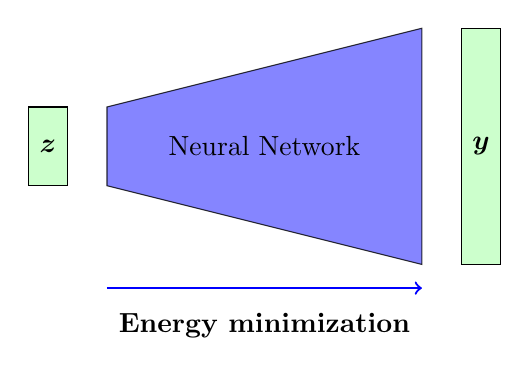
\begin{tikzpicture}
        % Modal coordinate (z)
        \draw[fill=green!20] (-3, 1) rectangle (-2.5,2);
        \node at (-2.75, 1.5) {$\bm{z}$}; % Label inside the rectangle
        
        % Displacement (u)
        \draw[fill=green!20] (2.5,0) rectangle (3,3);
        \node at (2.75, 1.5) {$\bm{y}$}; % Label inside the rectangle
        
        % Energy loss transition
        \draw[fill=blue!60,opacity=0.8] (-2,1) -- (2,-0) -- (2,3) -- (-2,2) -- cycle;
        \node at (0,1.5) {Neural Network};
        \node[below] at (0,-0.5) {\textbf{Energy minimization}};
        
        % Energy loss arrow
        \draw[thick,blue,->] (-2,-0.3) -- (2,-0.3);
    
    \end{tikzpicture}
    \caption{Neural Modes architecture for learning nonlinear deformation corrections}
    \label{fig:neural_modes_arch}
\end{figure}

\subsubsection{Training the Neural Modes}
The training process for the Neural Modes network is based on minimizing a combination of physics-based losses, rather than simply minimizing the prediction error against ground truth data. The key losses used in training are:

\begin{enumerate}
    \item \textbf{Energy Loss}: Minimizes the internal strain energy of the deformed configuration $E(\bm{X} + \bm{l} + \bm{y})$, where $\bm{X}$ is the rest position, $\bm{l}$ is the linear mode displacement given by $\bm{z}$, and $\bm{y}$ is the nonlinear correction.
    
    \item \textbf{Orthogonality Loss}: Ensures that the nonlinear correction is orthogonal to the linear mode space: $\bm{y}^T \bm{l} = 0$.
    
\end{enumerate}

The total loss function is a weighted sum of these individual losses:
\begin{equation}
    \text{Loss} = \text{Energy Loss} + \lambda_1 \text{Orthogonality Loss} + \lambda_2 \text{Origin Loss}
\end{equation}
where $\lambda_1$ and $\lambda_2$ are weight parameters that balance the importance of each loss term.

During the training process, it was observed that the network had the tendency to learn a correction when given \(z = 0\) (i.e., the rest position), and that was not intended, because the rest position should not have any correction, meaning that the model prediction should be zero. To avoid this, the network was designed to have zero bias, so that its output was centered at the origin.

\subsubsection{Dynamic Simulation with Neural Modes}
For dynamic simulations, the Neural Modes framework solves an optimization problem at each time step. Given the current and previous displacement states $\bm{u}_n$ and $\bm{u}_{n-1}$, the modal coordinates for the next time step $\bm{z}_{n+1}$ are computed by:
\begin{equation}
    \bm{z}_{n+1} = \underset{\bm{z}}{\argmin} \frac{1}{2h^2} \|\bm{n}(\bm{z}) - 2\bm{u}_n + \bm{u}_{n-1}\|_{\bm{M}}^2 + E(\bm{n}(\bm{z}))
\end{equation}
where $\bm{n}(\bm{z})$ represents the complete displacement field (linear modes plus nonlinear correction), $h$ is the time step, $\bm{M}$ is the mass matrix, and $E(\cdot)$ is the internal energy of the configuration. This optimization problem is typically solved using the L-BFGS-B algorithm.

One challenge with this approach is that the optimization problem does not explicitly account for external forces. The network learns to minimize internal energy but lacks direct information about external forces that may be applied during simulation. This limitation can affect the accuracy of dynamic simulations, particularly for large deformations or complex loading conditions.

\subsection{Extensions and Improvements}
A possible extension to the Neural Modes approach is to incorporate information about external forces directly into the network. This could be achieved by learning a mapping $\Phi: \mathbb{R}^m \rightarrow \mathbb{R}^n$ that relates modal coordinates $\bm{z}$ to the corresponding external forces $\hat{\bm{f}}$ that would produce such deformation. This additional network could be trained on a dataset of deformations and corresponding external forces, and then integrated into the dynamic simulation process to improve accuracy.

The objective function for dynamic simulation could then be extended to:
\begin{equation}
    \bm{z}_{n+1} = \underset{\bm{z}}{\argmin} \frac{1}{2h^2} \|\bm{n}(\bm{z}) - 2\bm{u}_n + \bm{u}_{n-1}\|_{\bm{M}}^2 + E(\bm{n}(\bm{z})) + \text{F}(\bm{z}, \bm{f})
\end{equation}
where $\text{F}(\bm{z}, \bm{f})$ is a term that accounts for the external forces acting on the system.

\section{Data driven correction}
\label{sec:dd_correction}

In this section will be presented the idea behind the method proposed to solve this problem. It is something that it's been already explored in the CFD world, although with some differences. 

It will be taken into account two discretization of the domain \(\Omega\), called \(\Omega_c\) and \(\Omega_f\) where the subscript \(c\) stands for ``coarse'' and the subscript \(f\) stands for ``fine''. The final goal is to have a solution on the coarse grid that is as close as possible to the solution on the fine grid. One possibility is to find a map \(G: \Omega_f \rightarrow \Omega_c\) that maps the solution on the fine grid to the coarse grid. 

The first solution that comes to mind is to use a neural network to find this map. So find an approximation \(\mathcal{NN}(\bm{u}) \approx G(\bm{u})\), by training the neural network on a dataset of pairs of solutions on the fine and coarse grid. This method has some drawbacks, the main one is that the neural network is trained on a fixed set of nodes, so if the coarse discretization changes, the method is not working anymore. The ideal solution for this problem is to have a model that is able to compute the solution for any given topology of the grid.

The problem with varying topologies is that the number of nodes of the mesh is not fixed, and this is a problem with Fully Connected Neural Networks (FCNN), where the input size is fixed. The need of a fixed input size can be solved by creating a fixed grid on each geometry, and then interpolate the solution on this grid. At this point, both the solutions on the fine and coarse grid are computed on the same grid. Having the solution on the same grid allows for multiple new possibilities, like computing the difference between the two solutions, a sort of ``error'' that is generated by the coarse grid. A neural network can be trained to learn this error and then correct the solution on the coarse grid, eliminating completely the need of the fine grid. In this way, the simulation can be run on the coarse grid, and then the neural network can be used to correct the solution, avoiding the ``black-box'' approach of having the model predicting a complete solution on a fine grid. This allows the method to be used also in a dynamical setting, avoiding the main problem that affects some existing methods. When a method tries to predict the temporal evolution of the system with deep learning techniques usually present the problem of accumulation of error, because the error at time-step \(t\) is carried over at time-step \(t+1\), and for a large number of time-steps this becomes noticeable and the prediction of the model is not accurate. 

This corrective method instead relies on the numerical solver for the temporal evolution of the problem, minimizing the accumulation of the error since it uses an exact method for the temporal evolution and the ``initial'' prediction before the correction from the model.

In a more formal way, the method can be described as follows. Let \(G \subset \Omega\) be a collection of points placed on a regular grid inside the domain \(\Omega\). Let \(\bm{u}_f\) be the solution of the problem on the fine grid and \(\bm{u}_c\) be the solution of the problem on the coarse grid. Once the two solution are computed, it is possible to take advantage of the FEM to interpolate the solution on the grid \(G\), obtaining \(\bm{u}_f^G\) and \(\bm{u}_c^G\). Now that both solutions live on the same grid, it is possible to compute the difference between the two solutions, obtaining the error \(\bm{e}^G = \bm{u}_f^G - \bm{u}_c^G\). The model is trained on the dataset \(\mathcal{D} = \{(\bm{u}_c^G, \bm{e}^G)\}\) to learn the error and then correct the solution on the coarse grid. The corrected solution is given by 
\[
    \hat{\bm{u}}_f^G = \bm{u}_c^G + \mathcal{NN}(\bm{u}_c^G).
\]
Once the model is trained, it can be used to correct the solution on the coarse grid, by interpolating back the solution on the original grid using Radial Basis Functions (RBF) interpolation. 


%-----------------------------------------------------------------------------
% CONCLUSION
%-----------------------------------------------------------------------------


%---------------------------------------------------------------------------
%  BIBLIOGRAPHY
%---------------------------------------------------------------------------
\newpage
\printbibliography
% Remember to insert here only the essential bibliography of your work
% automatically inserted and ordered with this command

\end{document}
